
MINRES法は,実対称またはエルミートな係数行列に対して有効な Krylov 部分空間法であり,
\textcolor{red}{Lanczos過程}に基づいて最小残差解を反復的に求める.

これをシフト線形方程式に拡張したのが shifted MINRES法(sminres)である.

アルゴリズムの概要: 
\vspace{-8pt}
\begin{enumerate}
	\item $A$に対して Lanczos過程を実行し,正規直交基底を構成
		\begin{align}
			\hspace{-2cm}
			AV_{n} = V_{n+1}\widehat{T}_{n},\ V_{n}=[\vb{v}_1 \ \cdots \ \vb{v}_n],\ T_{n} =
			{\small
			\begin{bNiceMatrix}[nullify-dots, columns-width=1.5em, cell-space-top-limit=5pt, cell-space-bottom-limit=5pt]
				\alpha_{1}	& \beta_{1}	&		&			\\
				\beta_{1}	& \Ddots	& \Ddots	& 			\\
    						& \Ddots	&		& \beta_{n-1}	\\
    						&		& \beta_{n-1}& \alpha_{n}		\\
			\end{bNiceMatrix}
			}
			,\ \widehat{T}_{n} = 
			{\small
			\mqty[T_{n} \\ \beta_{n}\vb{e}_{n}^{\top}]
			}
		\end{align}
	\item $k=1, 2, \dots, M$
	\begin{enumerate}
		\item $\widehat{T}_{n}^{(k)} = \widehat{T}_{n} + \sigma^{(k)} {\small \mqty[I \\ \vb{0}^\top]}$とおく($(A+\sigma^{(k)}I)V_{n}=V_{n+1}\widehat{T}_{n}^{(k)}$が成り立つ)
		\item $\widehat{T}_{n}^{(k)}$のQR分解を計算する($T_{n}^{(k)} = Q_n R_n$)
		\item $\vb{y}_{n}^{(k)} = \norm{\vb{b}} R_{n}^{-1} Q_{n}^{\htop} \vb{e}_{1}$を求める
			\begin{align}
				\| \vb{r}_n^{(k)} \|
				= \| \vb{b} - (A+\sigma_{k}I)\vb{x}_{n} \|
				&= \Bigl\| V_{n+1} \left( \|\vb{b}\| \vb{e}_1 - \widehat{T}_{n}^{(k)} \vb{y}_{n}^{(k)} \right) \Bigr\| \notag\\
				&= \Bigl\| \|\vb{b}\| \vb{e}_1 - \widehat{T}_{n}^{(k)} \vb{y}_{n}^{(k)} \Bigr\|
				\label{03-siki}
			\end{align}
		\item 最小残差解 $\vb{x}_{n}^{(k)} = V_{n} \vb{y}_{n}^{(k)}$を求める
	\end{enumerate}
\end{enumerate}
特徴:
\begin{itemize}
	\item \textcolor{red}{$1$回}のLanczos過程で\textcolor{red}{$M$個}の方程式に必要な基底が得られる
	\item \textcolor{red}{残差のノルムの単調減少性}と\textcolor{red}{無破綻性}を持つ
	\item シフトごとに\textcolor{red}{独立に}最小残差解を求められる
\end{itemize}

\vspace{0.5em}
\begin{figure}[H]
	\centering
	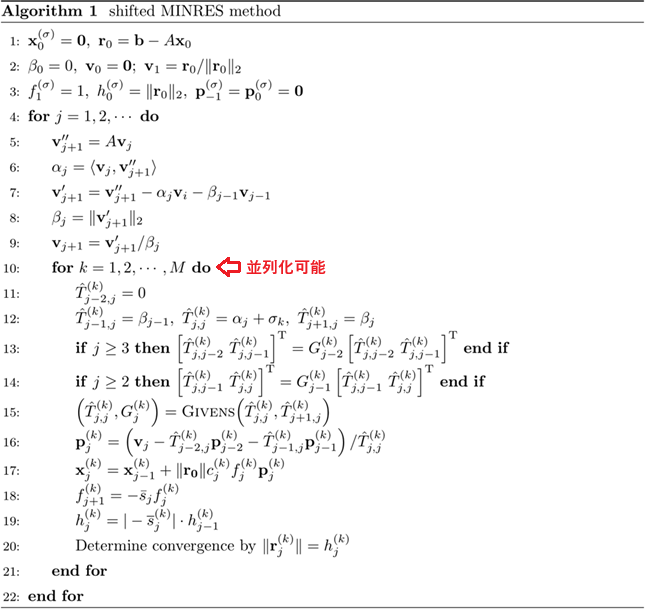
\includegraphics[scale=2.2]{./fig/algorithm-sminres.png}
\end{figure}



\begin{comment}
\begin{algorithm}[H]
	\caption{Multiply shifted MINRES algorithm}\label{Algorithm2}
	\begin{algorithmic}[1]
		\State ${\bf r}_0={\bf b}$, \, ${\bf q}_1 = {\bf r}_0/\|{\bf r}_0\|$, \, ${\bf p}_{-1}^{(m)}={\bf p}_0^{(m)}={\bf 0}$ \; ($m=1,\ldots,M$)
		\State $\beta_0=0$, \, $f_1^{(0,m)}=1$, \, $h_1^{(0,m)} = \|{\bf r}_0\|$ \; ($m=1,\ldots,M$)
		\For{$j=1, 2, \ldots,$}
			\State ${\bf q}_{j+1}^{\prime\prime} = A{\bf q}_j - \beta_{j-1}{\bf q}_{j-1}$
			\State $\alpha_j=\langle{\bf q}_{j+1}^{\prime\prime},{\bf q}_j\rangle$
			\State ${\bf q}_{j+1}^{\prime}={\bf q}_{j+1}^{\prime\prime}-\alpha_j{\bf q}_j$
			\State $\beta_j=\|{\bf q}_{j+1}^{\prime}\|$
			\For{$m=1,\ldots,M$}
				\State $r_{j-2,j}^{(m)}=0, \, r_{j-1,j}^{(m)}=\beta_{j-1}, \, r_{jj}^{(m)}=\alpha_j+\sigma^{(m)}$
				\State {\bf If} $j\ge 3$, update $r_{j-2,j}^{(m)}$ and $r_{j-1,j}^{(m)}$ by \eqref{eq:rkm2k}
				\State {\bf if} $j\ge 2$, update $r_{j-1,j}^{(m)}$ and $r_{jj}^{(m)}$ by \eqref{eq:rkm1k}
				\State compute $G_j^{(m)}$ and update $r_{jj}^{(m)}$ by \eqref{eq:rkk}
				\State ${\bf p}_j^{(m)}=({\bf q}_j-r_{j-2,j}^{(m)}{\bf p}_{j-2}^{(m)}-r_{j-1,j}^{(m)}{\bf p}_{j-1}^{(m)})/r_{jj}^{(m)}$
				\State ${\bf x}_j^{(m)}={\bf x}_{j-1}^{(m)} + \|{\bf r}_0\|c_j^{(m)} f_j^{(j-1,m)}{\bf p}_j^{(m)}$
				\State $f_{j+1}^{(j,m)}= -\bar{s}_j^{(m)} f_j^{(j-1,m)}$
				\State $h_{j+1}^{(j,m)}=|-\bar{s}_j^{(m)}| h_j^{(j-1,m)}$
			\EndFor
			\State ${\bf q}_{j+1}={\bf q}_{j+1}^{\prime}/\beta_j$
		\EndFor
	\end{algorithmic}
\end{algorithm}
\end{comment}